\paragraph{Analyse des résultats}:\\

Le but de cette section est d'analyser les résultats des expériences qu'on a mennées, afin de valider l'efficacité du passage à l'échelle du noyau d'ALMOS.\\
Les 3 premières figures illustrent les résultats en temps ( clocks ) et en nombre de mots ( en puissances de 2 ), pour chaque configuration ( 1, 4 et 16 clusters ), ces résultats montrent clairement que l'exécution multi-process est plus lente au début, ce qui signifie que la création et synchronisation des différents threads provoque des ralentissements de l'exécution multi par rapport à la mono, mais dès que le nombre de mots devient important, l'éxécution multi est largement plus efficace.\\
Le point intéressant dans ces graphes est donc celui du croisement des courbes multi et mono, là où la distribution des taches devient efficace :

\begin{center}
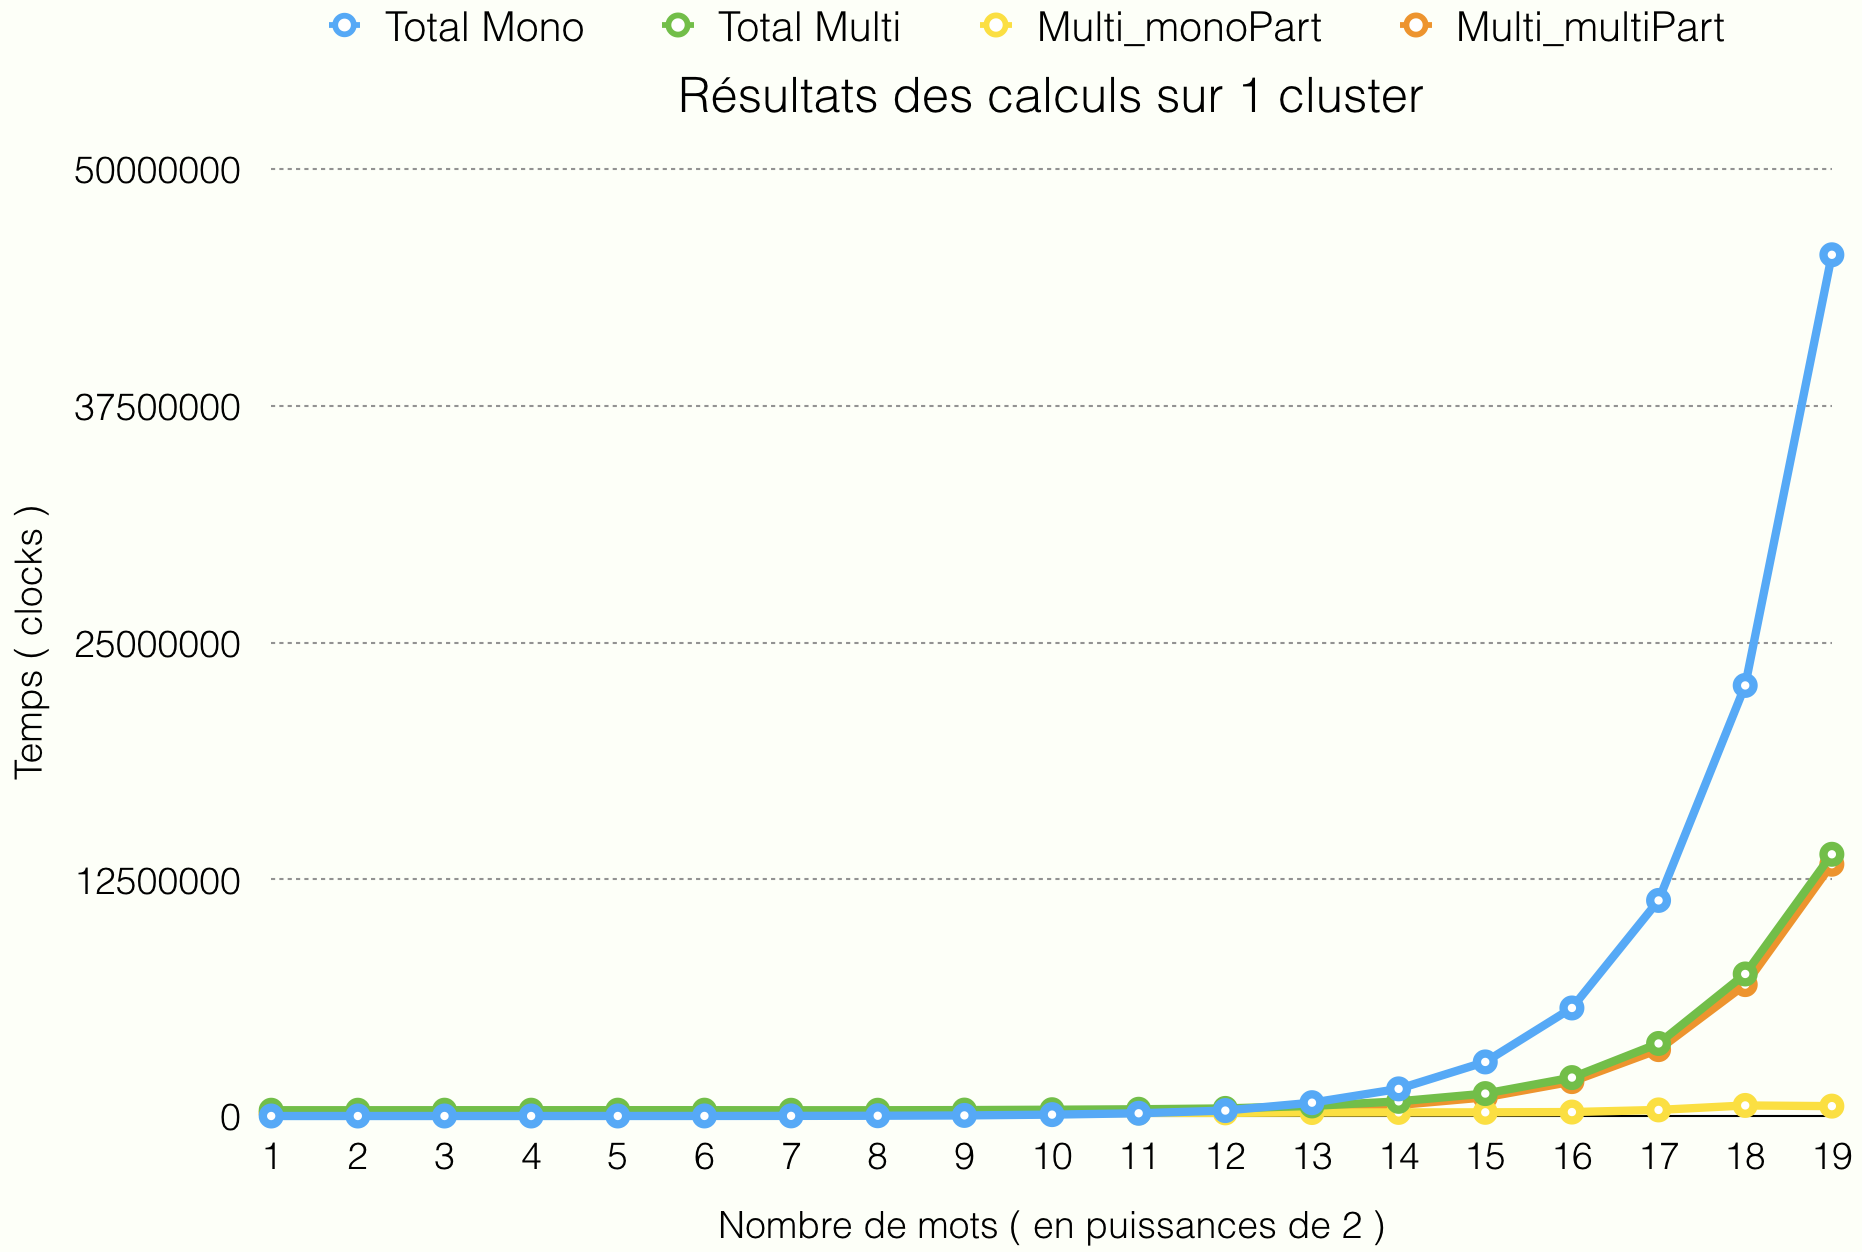
\includegraphics[scale=0.4]{images/graph_1.png}
\end{center}

\begin{center}
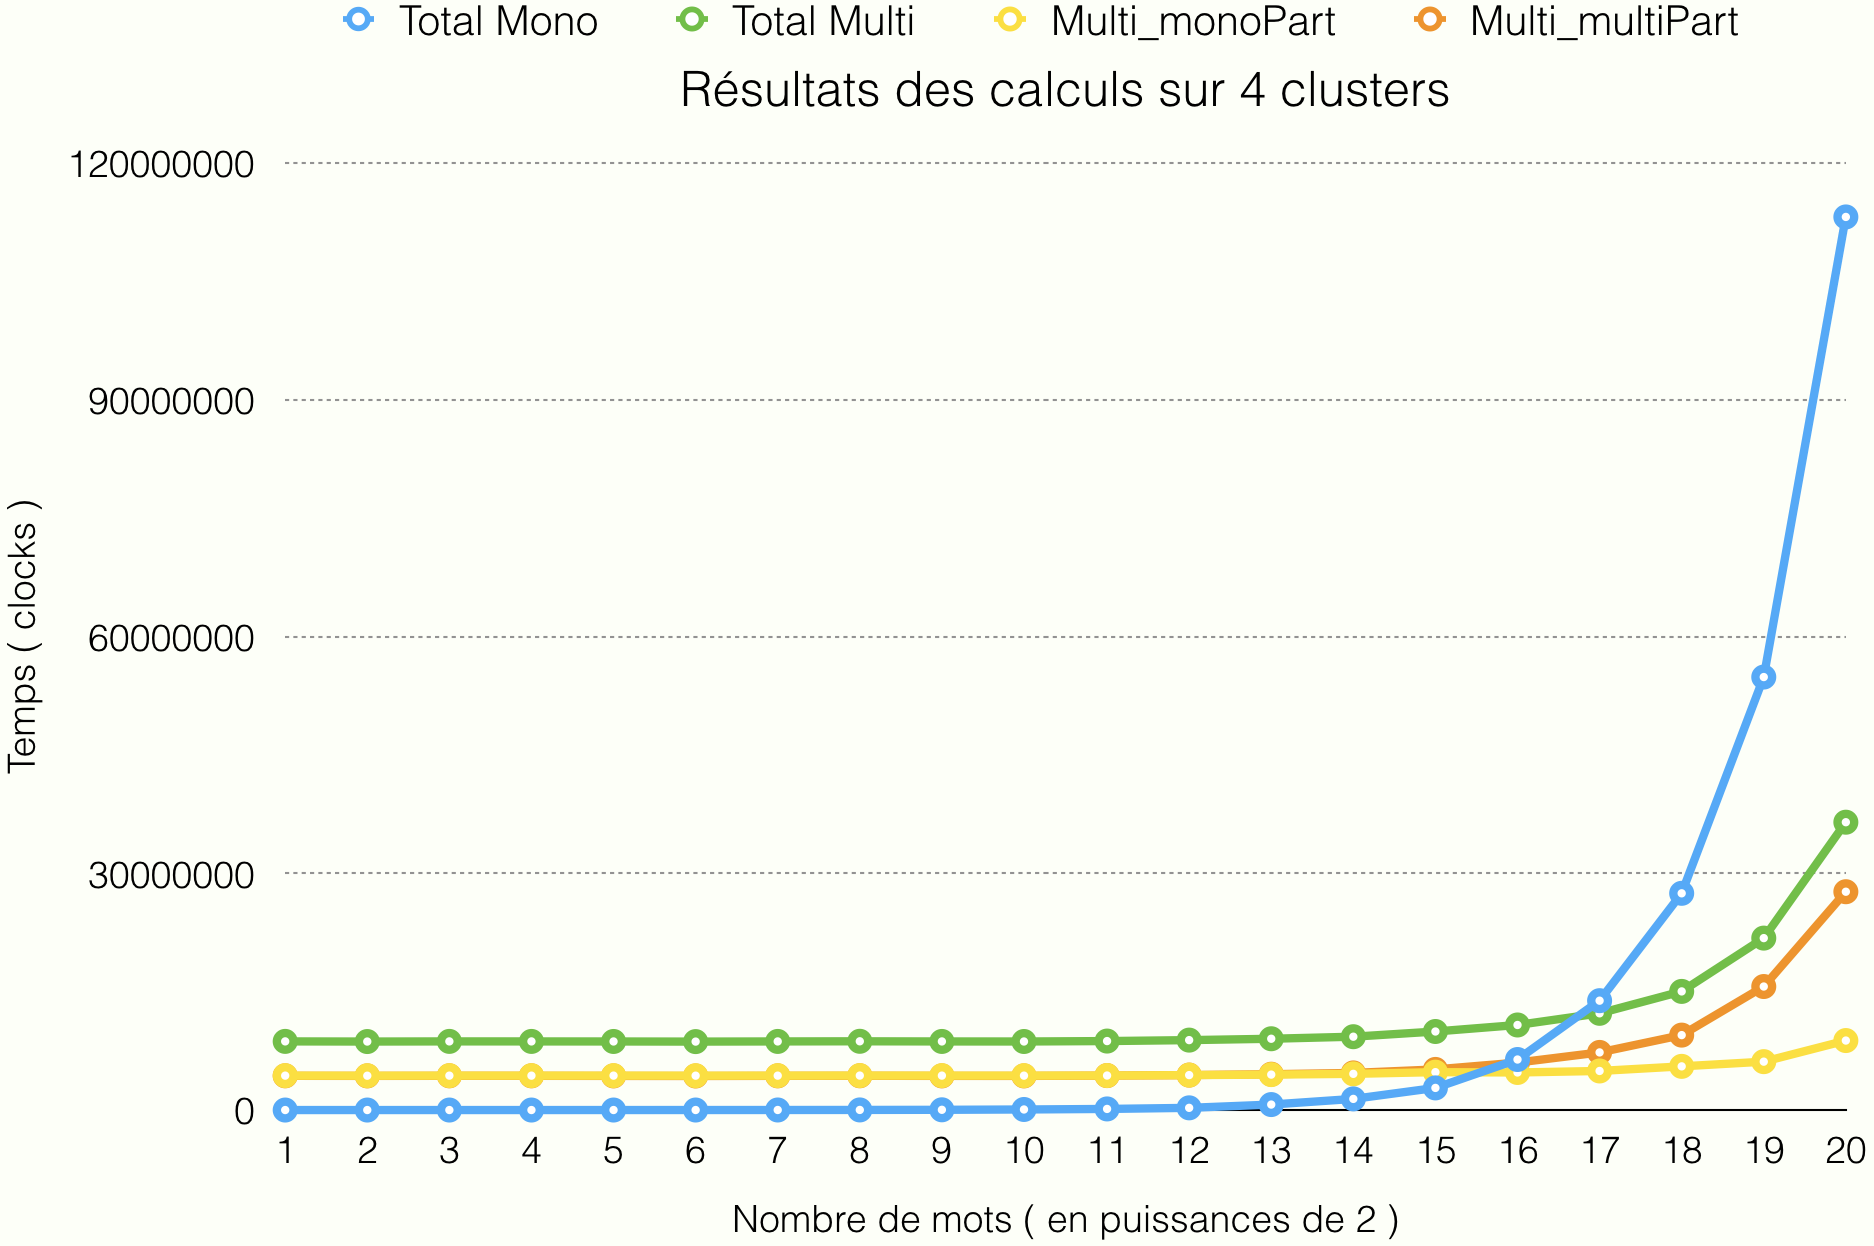
\includegraphics[scale=0.4]{images/graph_4.png}
\end{center}

\begin{center}
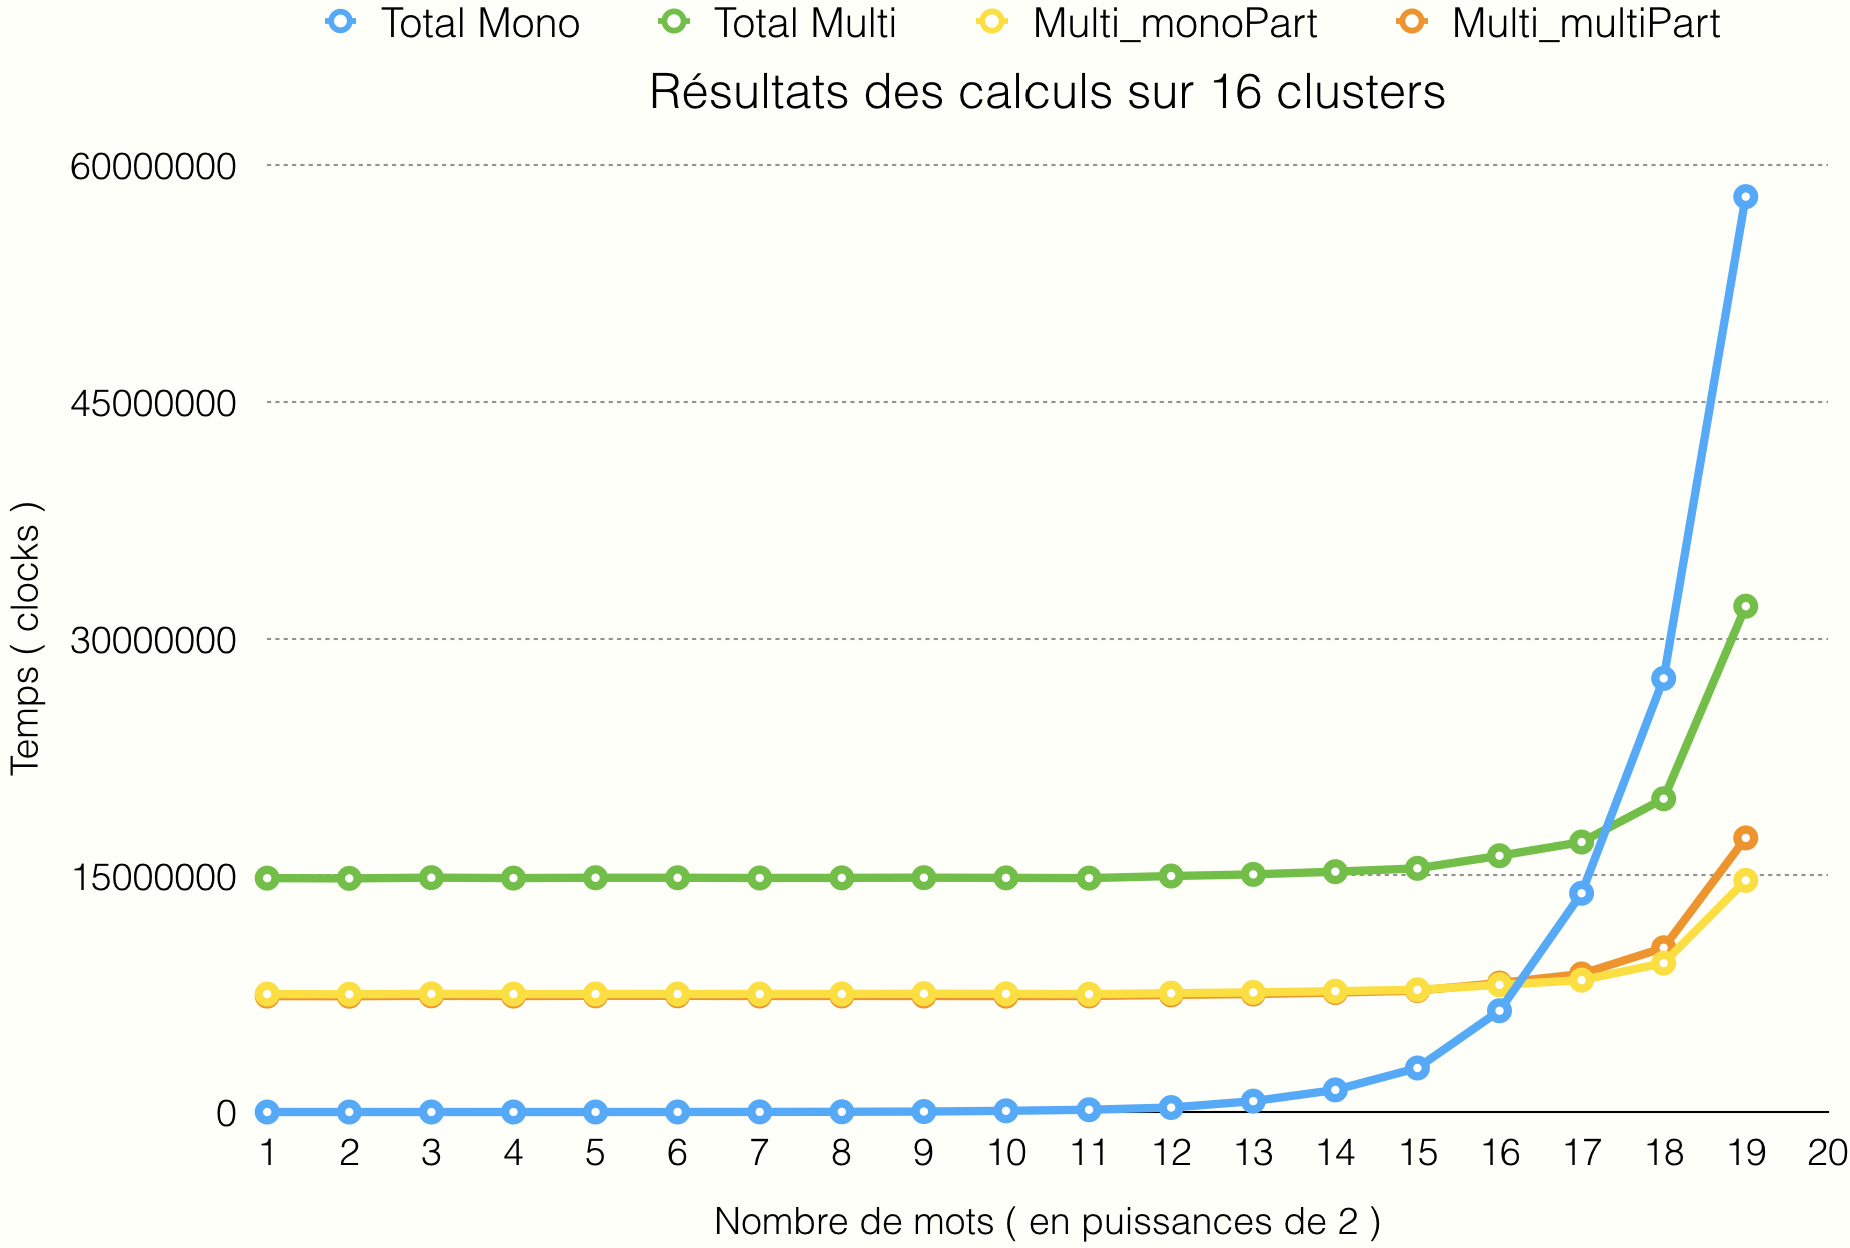
\includegraphics[scale=0.4]{images/graph_16.png}
\end{center}

On remarque également que, la différence en temps d'éxécution au départ est plus importante quand on a plus de coeurs, ce qui est normal vu la durée que prennent les différents coeurs pour leur initialisation, leur synchronisation ainsi que pour le déplacement des données ( auto-next-touch ).\\
Le point d'efficacité de la distribution des taches se trouve à 2\^12 pour 1 cluster, 2\^16 pour 4 clusters et 2\^17 pour 16 clusters.\\

Pour pouvoir évaluer l'efficacité de la distribution, et donc valider le passage à l'échelle en nombre de coeurs, on a réalisé un 4ème graphe représentant les Speed Up par configuration de clusters, c'est à dire le résultat obtenu pour chaque exécution, en appliquant un facteur ( Temps total en multi ) divisé par ( Temps total en mono ), ce qu'on a représenté dans la figure suivante :\\

\begin{center}
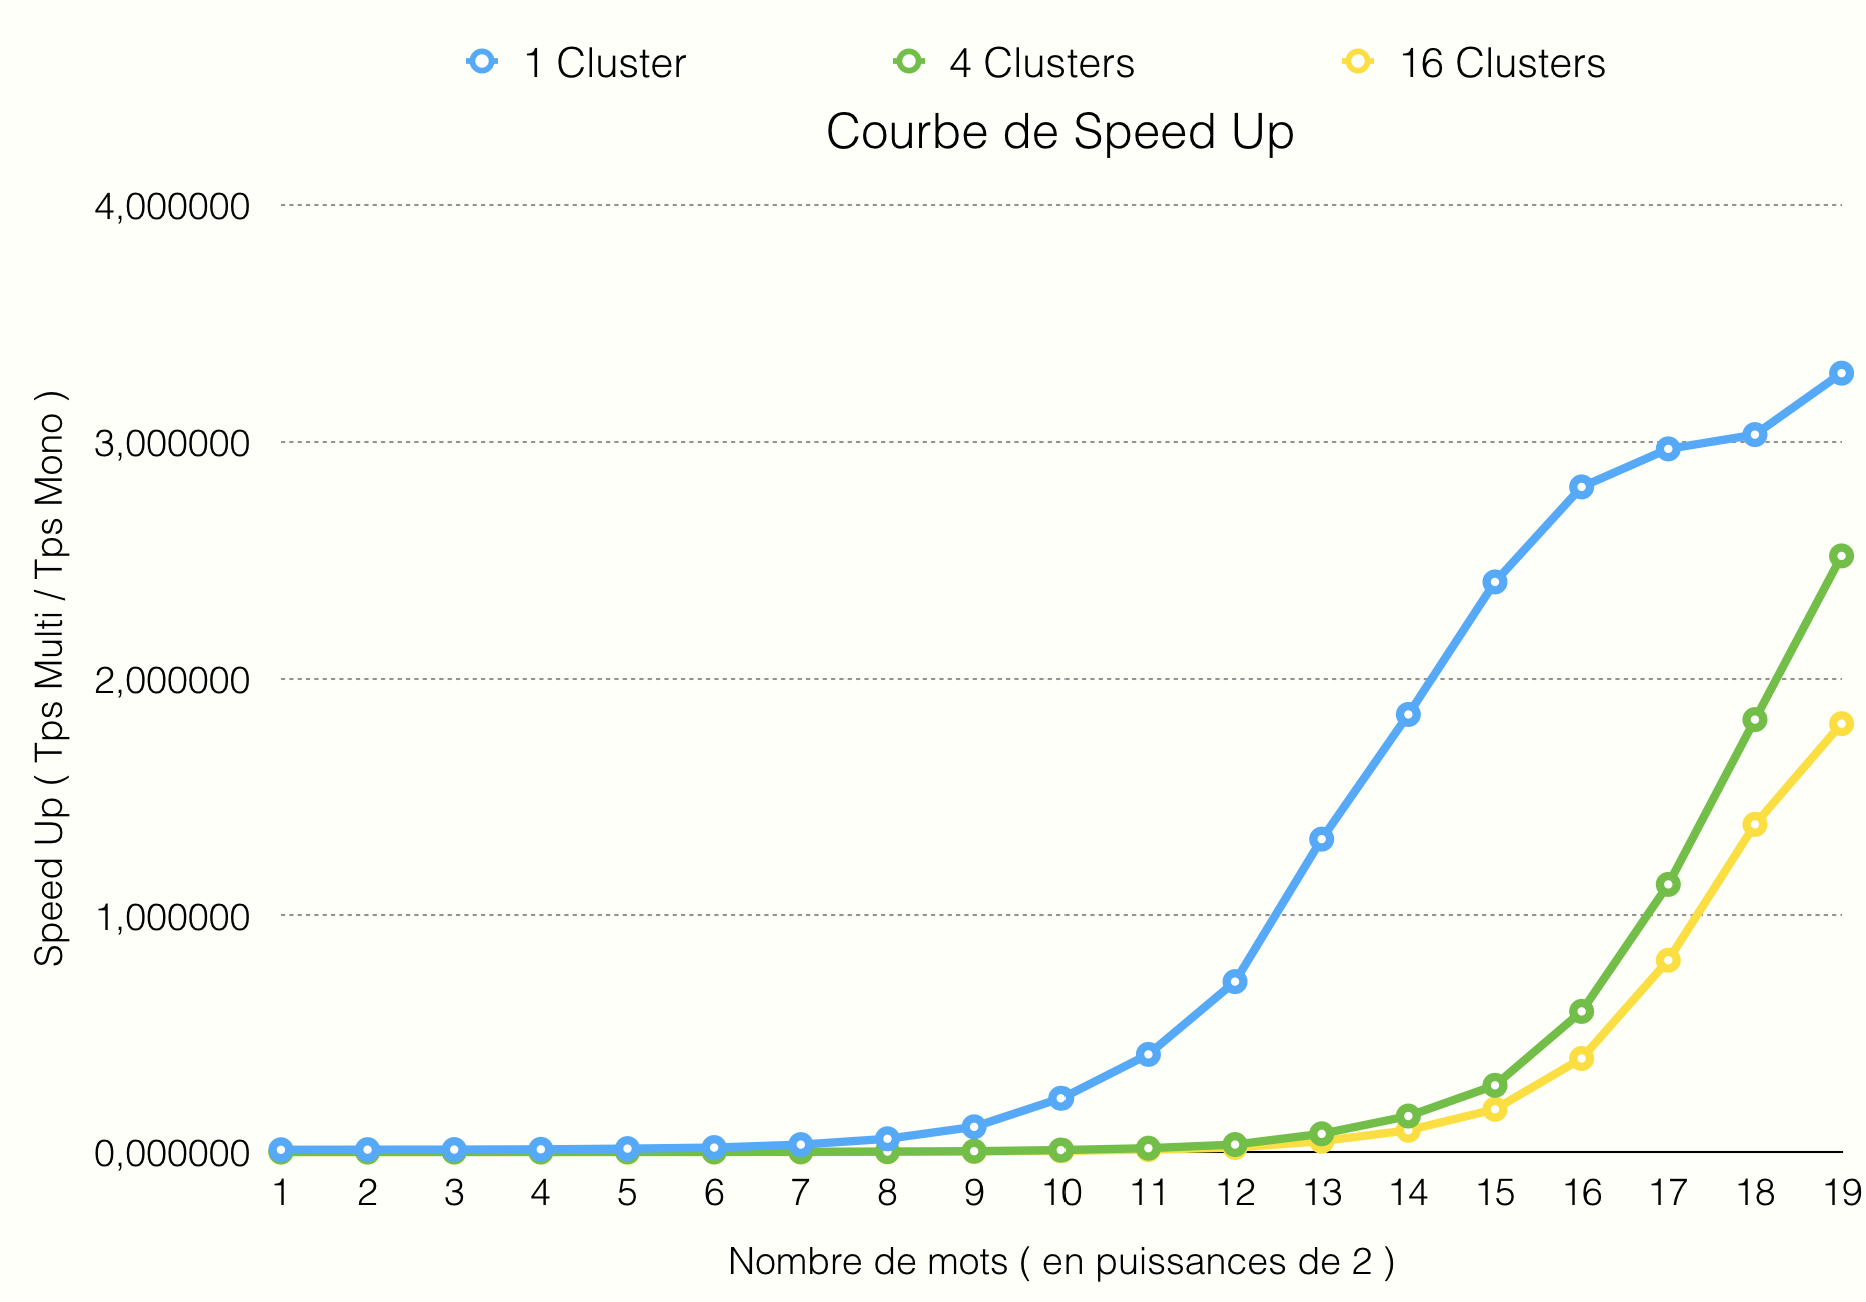
\includegraphics[scale=0.4]{images/graph_speedup.png}
\end{center}

Malheureusement, et pour des raisons que je n'ai pas réussi à identifier, on n'arrive pas à simuler
le programme pour plus de 1Mo de données, et du coup on a pas réussit à atteindre le point où
dans les courbes des SpeedUps le 16 serait plus efficace que le 4 qui serait plus efficace que le 1.
Notre expérimentation s'est donc arrêtée ici. Ce qui est un bon point d'avance par raport aux autres, d'après ce qu'on a pu constater.

\paragraph{Temps de simulation}:\\
La simulation a du prendre pour l'ensemble des configurations a du prendre 2 semaines sur les
machines de la fac.
